% Section content template for individual Educative lessons
% This file contains the actual content for a specific section
% Generated from Educative API section content

% Section: Class Diagram for the Hotel Management System
% Section ID: 6101784200478720
% Section Slug: class-diagram-for-the-hotel-management-system
% Generated: 2025-12-12T16:23:26.724932

Here, we will create the class diagram for our system based on the requirements we gathered in one of the previous lessons. In the class diagram, we will first design and create the classes, abstract classes, and interfaces for the system, and then we'll identify the relationship between classes in accordance with all the requirements of the hotel management system.

\subsection{Components of a hotel management system}\label{sFG-z80byCAKUNVj5oIGL}
\\
In this section, we'll define the classes for a hotel management system. Following the bottom-up approach to designing a class diagram, we will first create the classes of small components. Next , we will integrate these components and create the class diagram for the hotel management system.

\subsubsection{Address and Account}\label{92kRYcla_3ODBj7T0gXjC}
\\
The \texttt{Address} class is required to store any address. It is a custom data type with attributes like a street address, city, etc. In the hotel management system, this class will be used to specify the addresses of the users and the hotel.
\\
\texttt{Account} is a class used to store the user's account information. This class has three members, i.e., account ID, password, and account status. The class representation of \texttt{Address} and \texttt{Account} classes is as follows:

\begin{figure}[htbp]
 \centering
 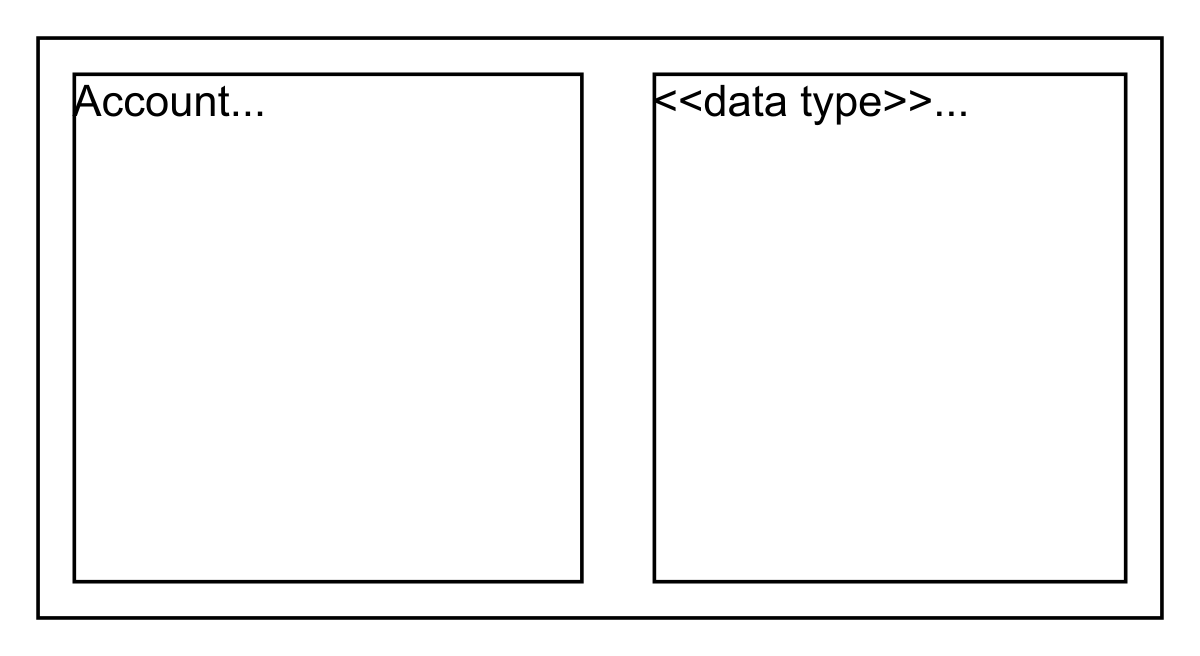
\includegraphics[width=0.5\textwidth]{Images/chapter_18/section_6101784200478720/5754278971834368.png}
 \caption{The class diagram of the Address and Account classes}
\end{figure}

\subsubsection{Person}\label{RmMg5DmgsexUkULnUt5st}
\\
\texttt{Person} is an abstract class used to store information related to a person, such as a name, email, phone number, etc. In this class, an object of the \texttt{Address} type specifies the person's address. The \texttt{Person} class specifies the accounts in the system. The system has four types of accounts: housekeeper, receptionist, guest, and server.
\\
There are multiple functions of the \texttt{Person} class's subclasses. First , the \texttt{Housekeeper} class will keep track of the maintenance records of a room. Second
, the \texttt{Receptionist} class represents the hotel receptionist. The methods in this class depict the actions that the receptionist can perform. Moreover , the \texttt{Guest} class describes the guests of the hotel. Guests are the hotel's customers who can search for and book a room.
\\
The relationship diagram for these classes is shown below:

\begin{figure}[htbp]
 \centering
 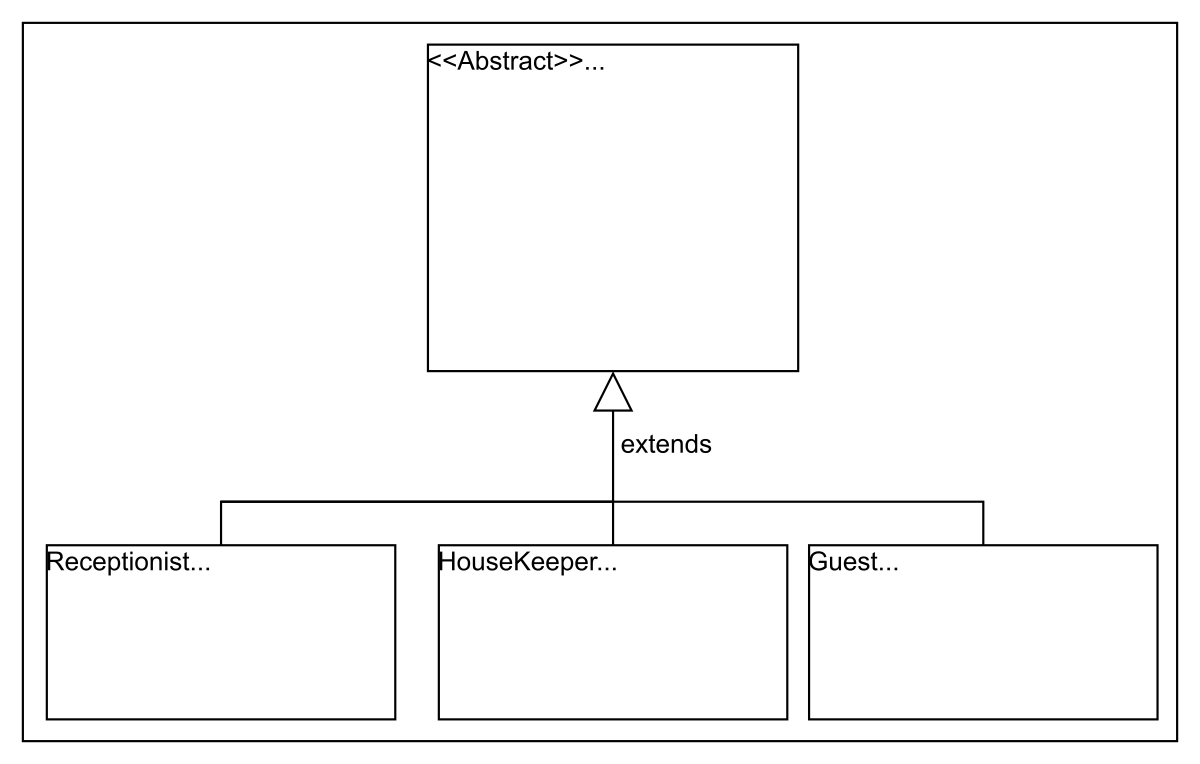
\includegraphics[width=0.5\textwidth]{Images/chapter_18/section_6101784200478720/6060629168095232.png}
 \caption{The class diagram of Person and its derived classes}
\end{figure}

\textbf{R1:} The system can have four types of accounts, such as housekeeper, receptionist, guest, or server.

\subsubsection{Service}\label{RaL7OUsivwIviWcLABJne}
\\
\texttt{Service} is an abstract class that encapsulates the details of different types of services guests have requested. Three types of services are provided: amenity, room service, and kitchen service.
\\
The \texttt{Amenity} class is a subclass of \texttt{Service} with two members: name and description. Similarly , \texttt{RoomService} is also inherited from the \texttt{Service} class. This class stores information about room services, whether these services are chargeable or not, and the request time of the service. Furthermore
, the last child class of the \texttt{Service} is \texttt{KitchenService}. The relationship between these classes is shown in the illustration below.

\begin{figure}[htbp]
 \centering
 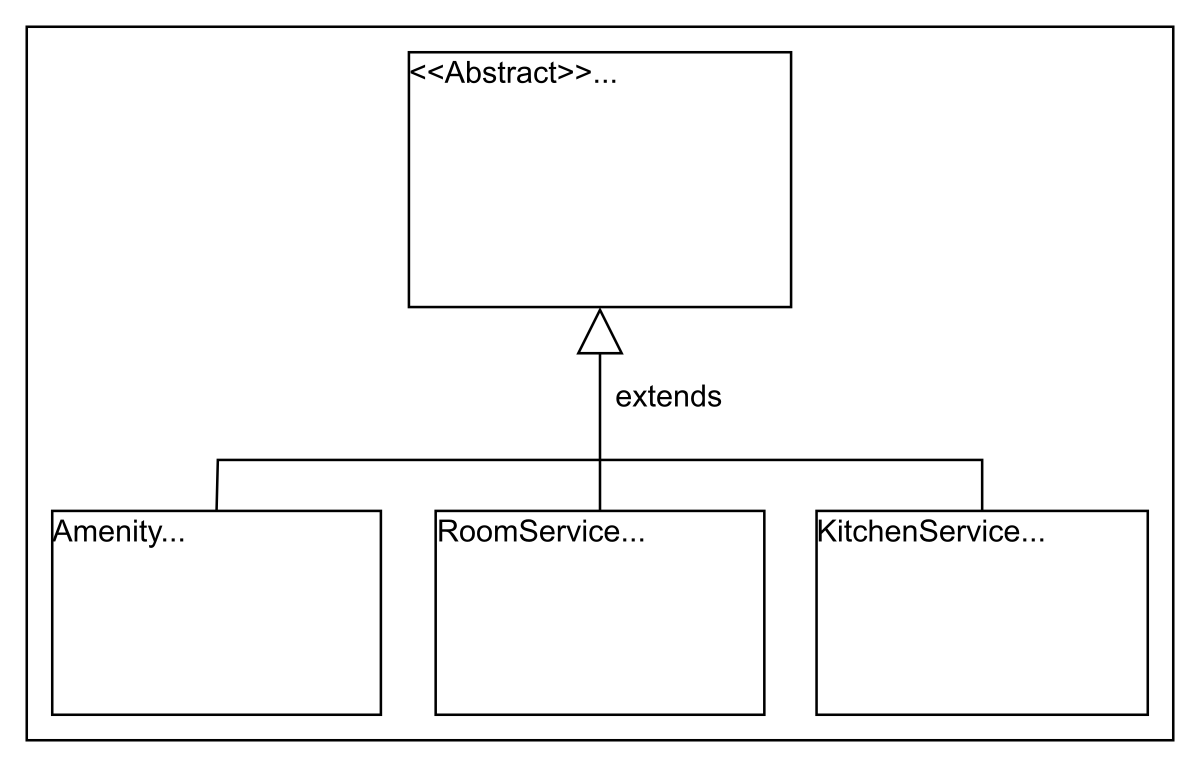
\includegraphics[width=0.5\textwidth]{Images/chapter_18/section_6101784200478720/4815403606736896.png}
 \caption{The class diagram of Service and its derived classes}
\end{figure}

\textbf{R8:} The system should allow customers to add services of their choice, such as room service, food or kitchen service, or amenities.

\subsubsection{Invoice}\label{unp3y-QDa6psC3OH52thY-2}
\\
The \texttt{Invoice} class represents the billing system in the hotel management system. The UML diagram for both classes is presented below:

\begin{figure}[htbp]
 \centering
 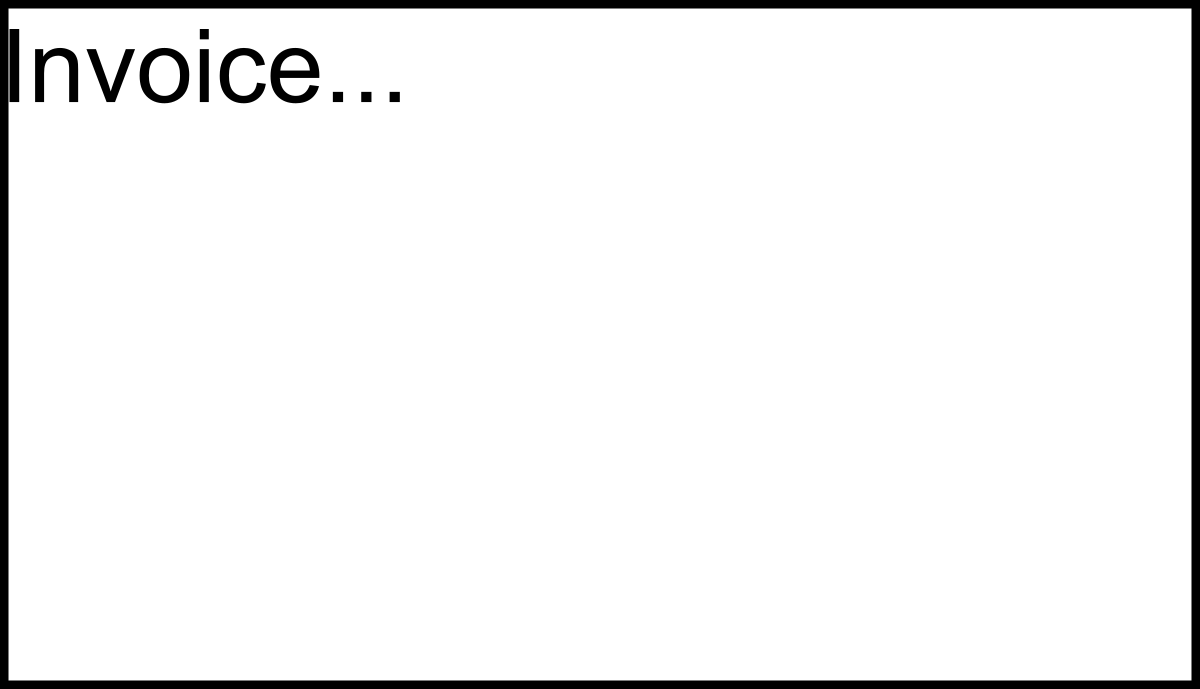
\includegraphics[width=0.5\textwidth]{Images/chapter_18/section_6101784200478720/4942337195376640.png}
 \caption{The class diagram of the Invoice class}
\end{figure}

\subsubsection{Room booking}\label{unp3y-QDa6psC3OH52thY-3}
\\
The \texttt{RoomBooking} class is responsible for managing the bookings for a room. This class includes attributes like reservation number, start date, duration, etc. Moreover , this class has a member of the \texttt{BookingStatus} type that is used to store the status of the room booking. The
UML representation of this class is as follows:

\begin{figure}[htbp]
 \centering
 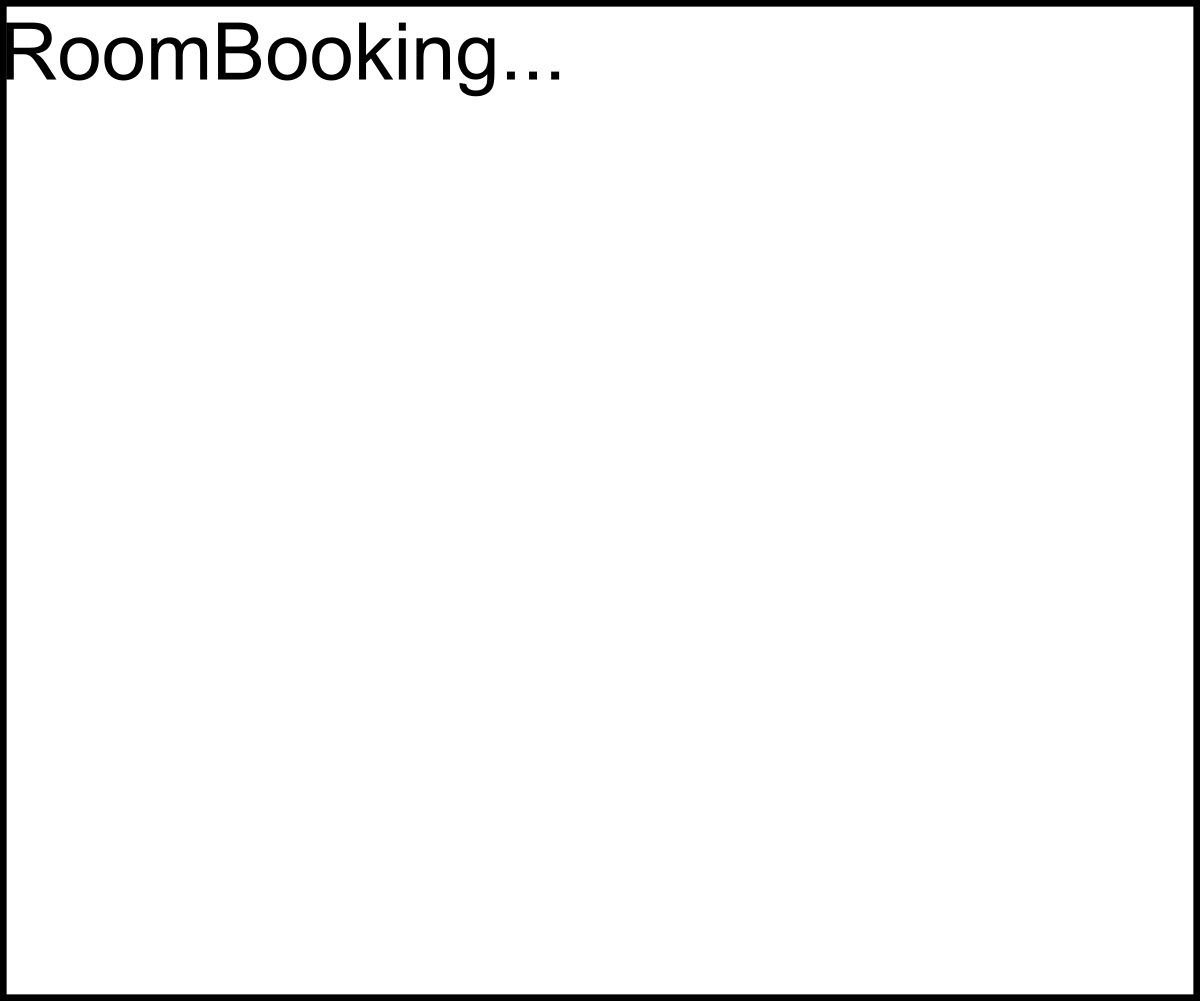
\includegraphics[width=0.5\textwidth]{Images/chapter_18/section_6101784200478720/5273457329963008.png}
 \caption{The class diagram of the RoomBooking class}
\end{figure}

\textbf{R4:} During room booking, the user enters the check-in date and duration of the stay. The user also has to make an advance payment.

\subsubsection{Notification}\label{FFhaZfzNUbPLfoFvRnC3-}
\\
\texttt{Notification} is an abstract class responsible for sending notifications to guests whenever the booking is nearing the check-in or check-out date. Every notification has an ID, creation date, and content. The notification can either be an SMS notification or an email notification.
\\
The \texttt{SMSNotification} class requires the member's phone number to send a notification. On the other hand, the \texttt{EmailNotification} needs the member's email address to send a notification. The relationship diagram of these classes is shown here:

\begin{figure}[htbp]
 \centering
 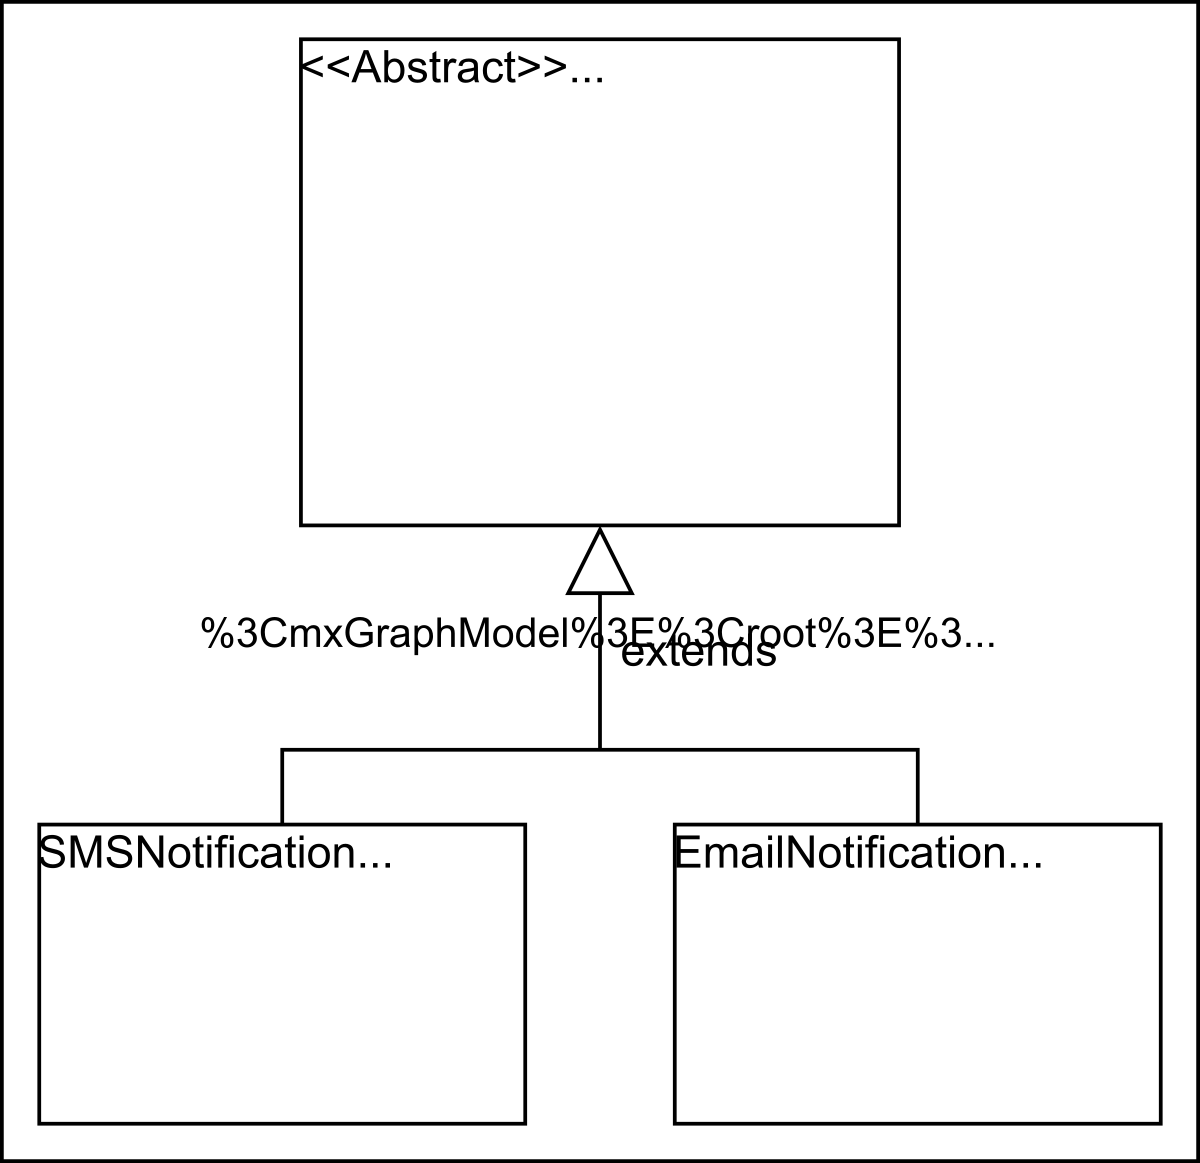
\includegraphics[width=0.5\textwidth]{Images/chapter_18/section_6101784200478720/5535276942491648.png}
 \caption{The class diagram of Notification and its derived classes}
\end{figure}

\textbf{R6:} The system should notify customers about the booking status or other information.

\subsubsection{Room, room key, and room maintenance}\label{P4z8rT5n_HGoR9L5X9bLr}
\\
The \texttt{Room} class is the system's basic building block. Every room has a room number and a price associated with it. The
\texttt{Room} class uses the \texttt{RoomStyle} and \texttt{RoomStatus} enums to specify the rooms' style and status, respectively.
\\
Each room has an electronic key card associated with it. The \texttt{RoomKey} class expresses the electronic key card. Each card has its own unique ID and barcode. The
\texttt{RoomKey} class also has members to store the issue date, to check whether or not the key is active, and to check whether or not a key is a master key. Whereas
, \texttt{RoomMaintenance} is a class used to keep track of all maintenance records for the rooms. The UML representation of these classes is as follows:

\begin{figure}[htbp]
 \centering
 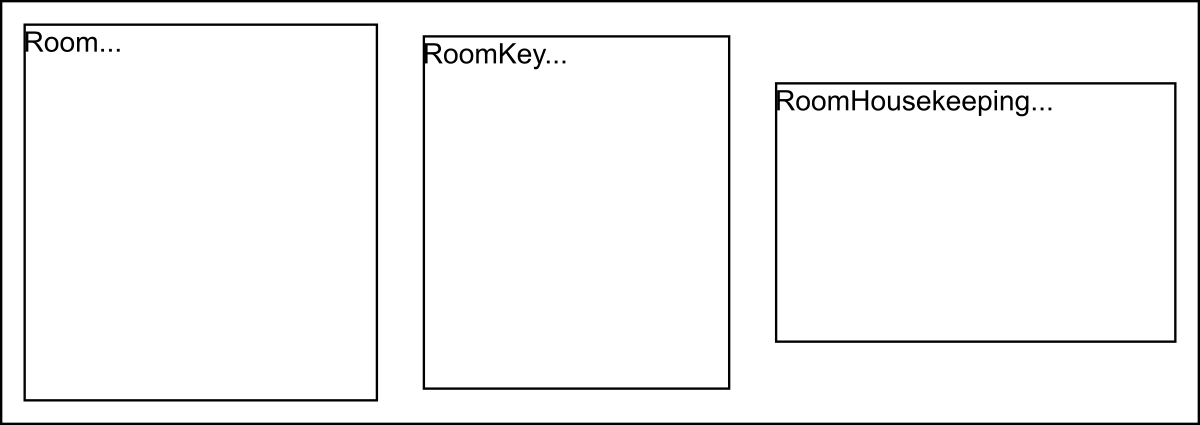
\includegraphics[width=0.5\textwidth]{Images/chapter_18/section_6101784200478720/5125013297692672.png}
 \caption{The class diagram of the Room, RoomKey, and RoomMaintenance classes}
\end{figure}

\textbf{R9:} Every room should have its specific key, and there can be a master key that opens a specific set of rooms.
\\
\textbf{R7:} The system should log and manage all the cleanup tasks.

\subsubsection{Search interface and catalog}\label{U_w2glMp6e3DkE6231op0}
\\
\texttt{Search} is one of the most important components of the hotel management system. In the diagram below, \texttt{Search} is the interface that allows guests to search for any room of their choice and pay range. The receptionist can also use this interface to search for any room. The \texttt{Catalog} class contains a list of all rooms and implements the \texttt{Search} interface.
\\
The following UML diagram shows this relationship:

\begin{figure}[htbp]
 \centering
 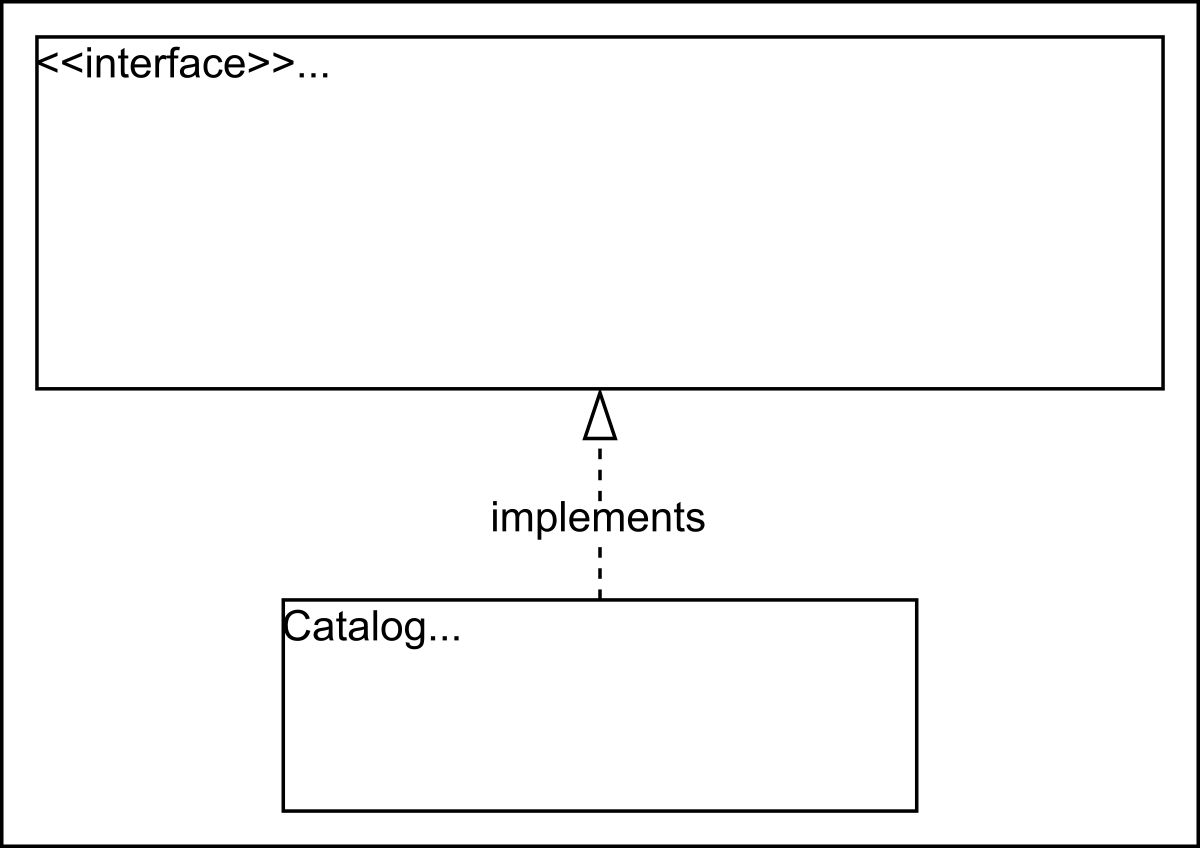
\includegraphics[width=0.5\textwidth]{Images/chapter_18/section_6101784200478720/5034593700020224.png}
 \caption{The class diagram of the Search interface and the Catalog class}
\end{figure}

\textbf{R3:} The system should allow guests to search for and book any available room.

\subsubsection{Bill transaction}\label{au43LBmdmxgGADrsP9lZ3}
\\
After generating an invoice, a customer must pay the bill to confirm the room booking. A \texttt{BillTransaction} class is required to store the information of bill payment. Check , cash, and credit card transactions are three ways to pay the bill. We can define the bill payment functionality through any payment method using the diagram below:

\begin{figure}[htbp]
 \centering
 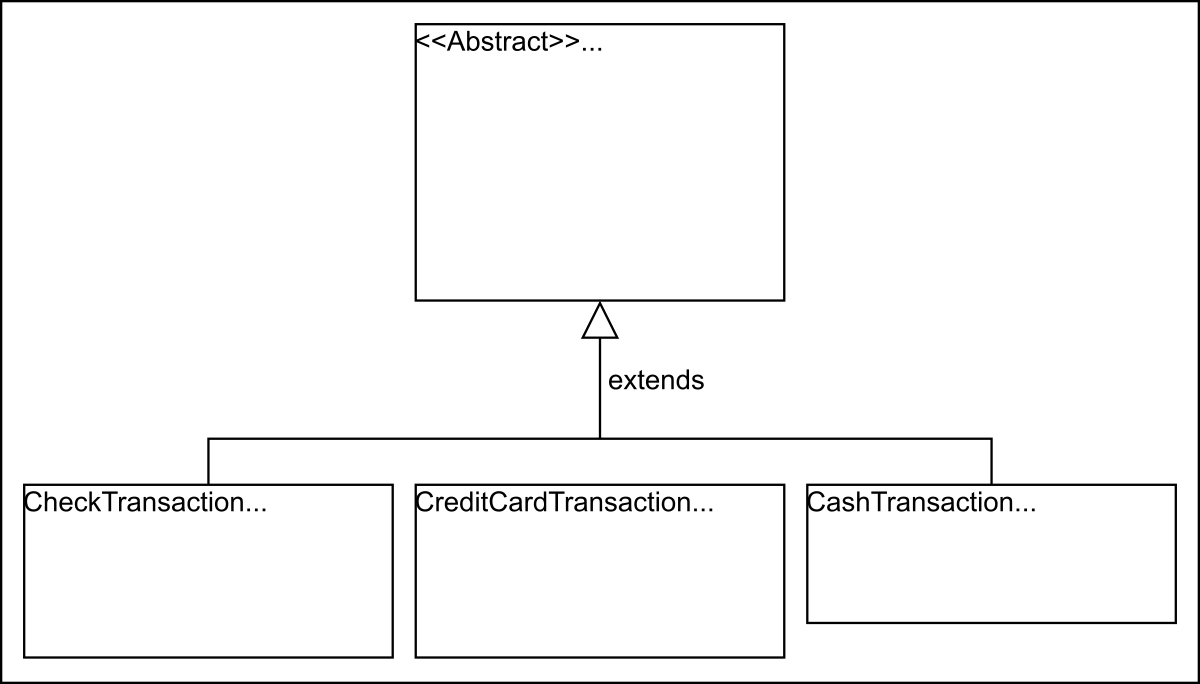
\includegraphics[width=0.5\textwidth]{Images/chapter_18/section_6101784200478720/5133484747390976.png}
 \caption{The class diagram of BillTransaction and its derived classes}
\end{figure}

\subsubsection{Hotel and hotel branch}\label{3YbTwqUHUvOZCk4TfFN4o}
\\
In this section, we'll look at the \texttt{Hotel} and \texttt{HotelBranch} classes. According to the requirements, there can be multiple branches of the hotel. \texttt{HotelBranch} is a class used to represent the location of the hotel branch. This class consists of two members: \texttt{name} and \texttt{Address}. The string type \texttt{name} is used to store the name of the hotel branch, while the complex object \texttt{Address} is used to store the complete address of a branch.
\\
The \texttt{Hotel} class is the base class of the system, which is used to represent the hotel. The visual representation of these classes is as follows:

\begin{figure}[htbp]
 \centering
 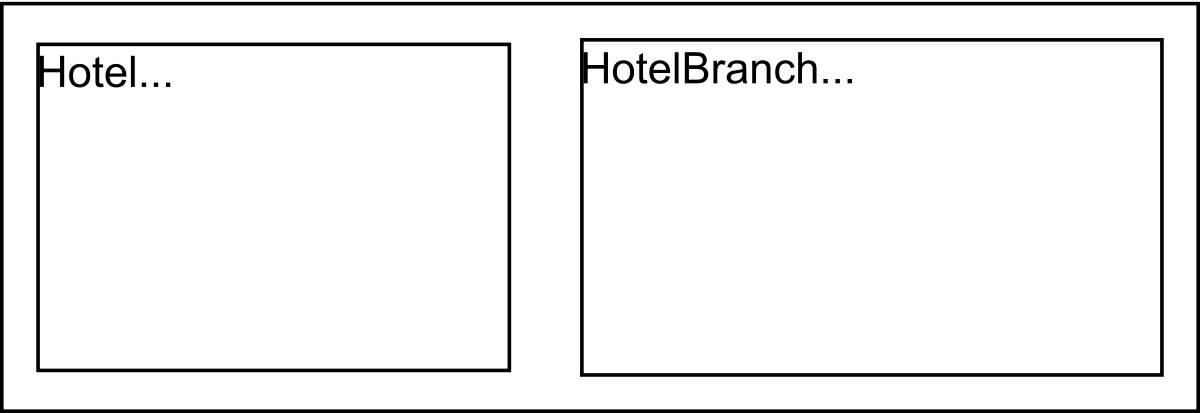
\includegraphics[width=0.5\textwidth]{Images/chapter_18/section_6101784200478720/6575481648578560.png}
 \caption{The class diagram of the Hotel and HotelBranch classes}
\end{figure}

\textbf{R10:} A hotel can have multiple branches.

\subsubsection{Enumerations}\label{unp3y-QDa6psC3OH52thY-4}
\\
Here is the list of enumerations required in the hotel management system:
\\
\texttt{BookingStatus}\textbf{:} This status describes the booking status, whether the booking is requested, pending, confirmed, canceled, or abandoned.
\\
\texttt{PaymentStatus}\textbf{:} This status describes the status of the booking's payment, whether it is unpaid, pending, completed, failed, declined, canceled, abandoned, setting, settled, or refunded.
\\
\texttt{RoomStatus}\textbf{:} This status describes the room's status, whether it is available, reserved, occupied, not available, being serviced, or any other possibility.
\\
\texttt{RoomStyle}\textbf{:} This describes the style of the room that the user wants to book. The style could be standard, deluxe, family, or business.
\\
\texttt{AccountStatus}\textbf{:} This status tells the status of the user account, whether it is active, closed, canceled, or blocklisted.
\\
\texttt{AccountType}\textbf{:} The account type tells the type of the user's account, whether it is a member, guest, manager, or receptionist.

\begin{figure}[htbp]
 \centering
 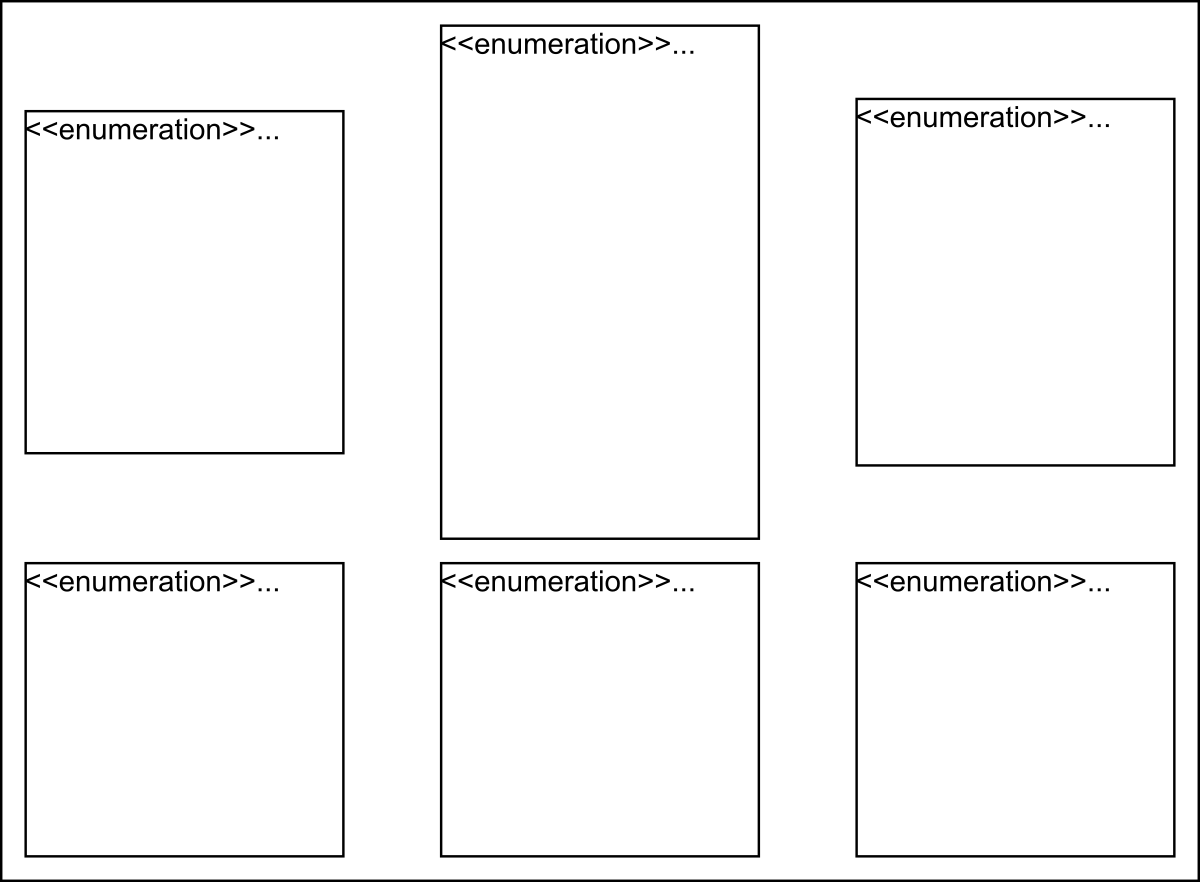
\includegraphics[width=0.5\textwidth]{Images/chapter_18/section_6101784200478720/6393659568422912.png}
 \caption{Enums in the hotel management system}
\end{figure}

\textbf{R2:} The rooms can be of different styles, such as standard, deluxe, family suite, or business suite.

\subsection{Relationship between the classes}\label{TQeQvn7wVlq23DuZpRwW7}
\\
Now, we'll discuss the relationships between the classes we have defined above in our hotel management system.

\subsubsection{Association}\label{irE7v5zwrnf2fGctATose}
\\
The class diagram has the following association relationships:
\\
\paragraph{One-way association}\label{yNslhiLgdT10nAnUhJ2Ck}

\begin{itemize}
\item
\protect\phantomsection\label{Rb4TEiK6d_dDKxGRV0HRt}
The \texttt{Housekeeper} class has a one-way association with \texttt{RoomMaintenance}.
\item
\protect\phantomsection\label{mBKZ0w91AF00ErvRPyET_}
Both \texttt{Receptionist} and \texttt{Guest} have a one-way association with \texttt{RoomBooking}.
\item
\protect\phantomsection\label{XBi6FupbiIae573xbaMi7}
The \texttt{RoomBooking} class has a one-way association with \texttt{Room}.
\end{itemize}

\begin{figure}[htbp]
 \centering
 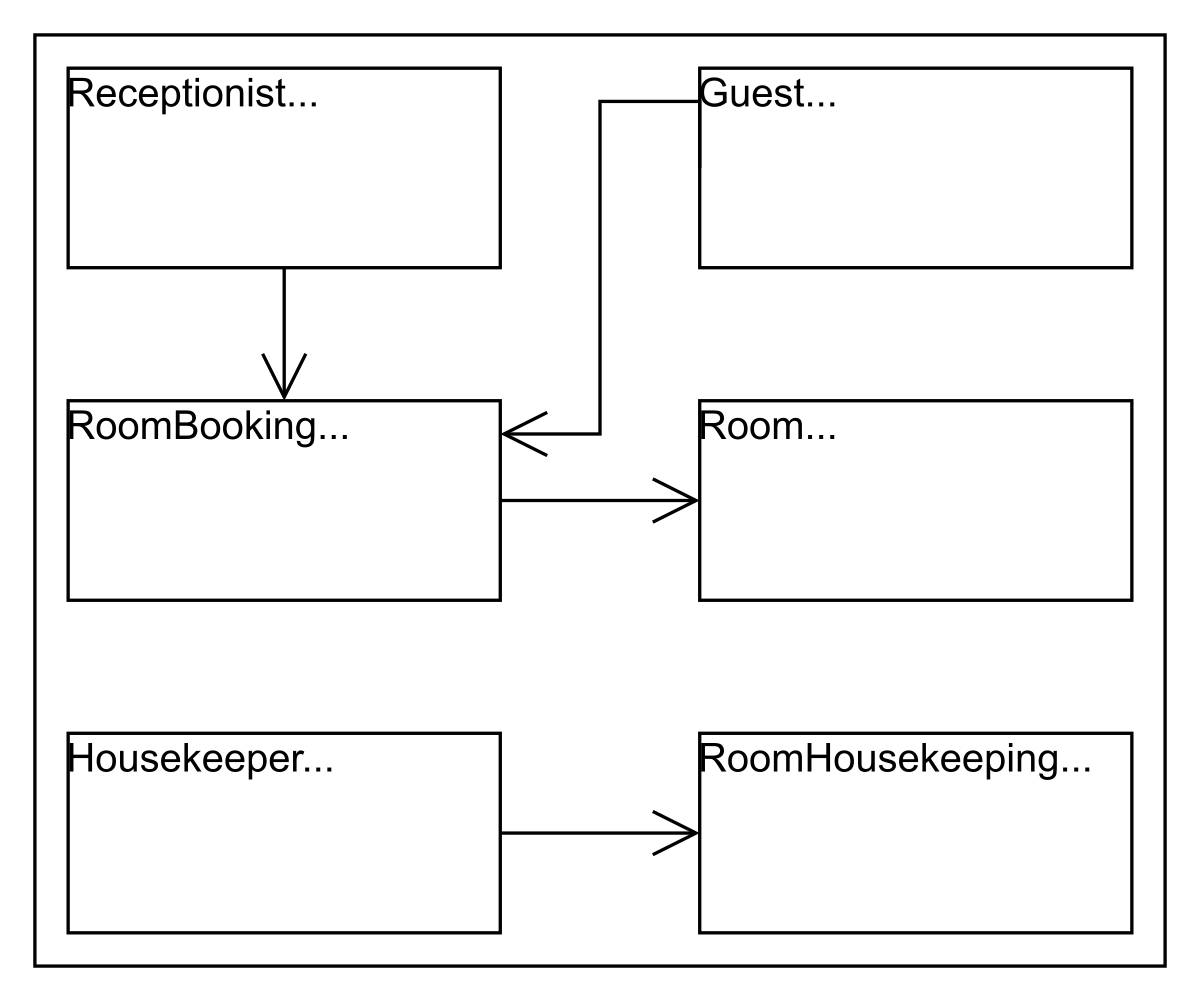
\includegraphics[width=0.5\textwidth]{Images/chapter_18/section_6101784200478720/5522715659075584.png}
 \caption{A one-way association relationship between classes}
\end{figure}

\paragraph{Two-way association}\label{A5aJabd4t9ShMc8TdNlWe}
\\
The \texttt{RoomBooking} class has a two-way association with \texttt{Notification}.

\begin{figure}[htbp]
 \centering
 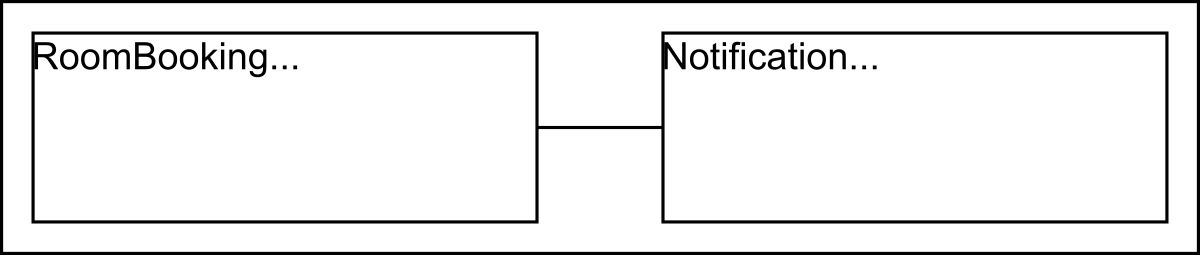
\includegraphics[width=0.5\textwidth]{Images/chapter_18/section_6101784200478720/5776268211781632.png}
 \caption{A two-way association relationship between classes}
\end{figure}

\subsubsection{Aggregation}\label{GrRDd34coTgbIpqCD8jOl-1}

\begin{itemize}
\item
\protect\phantomsection\label{PfujwBBWWIQrPsyiOhhLI}
The \texttt{RoomBooking} class is an aggregate of \texttt{Service}.
\end{itemize}

\begin{figure}[htbp]
 \centering
 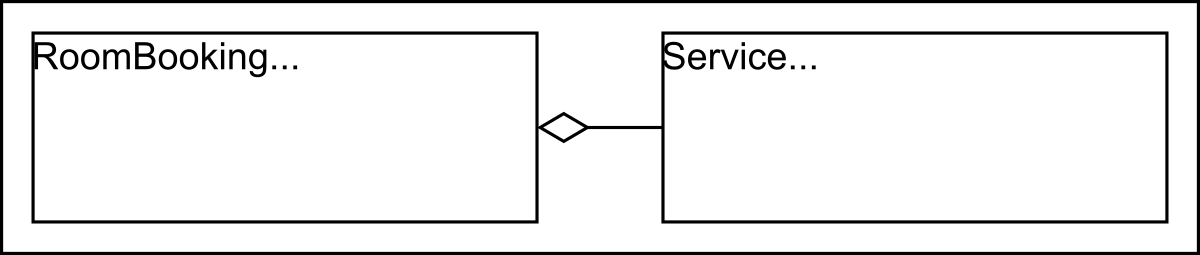
\includegraphics[width=0.5\textwidth]{Images/chapter_18/section_6101784200478720/5490737947082752.png}
 \caption{An aggregation relationship between classes}
\end{figure}

\subsubsection{}\label{l_Khl-QEMe0-pHuaf_qWt}

\subsubsection{Composition}\label{D-k4pyc7rwt5gmOf3YXA3}

\begin{itemize}
\item
\protect\phantomsection\label{ayVyYX-M9a2R_PieaXV5Q}
The \texttt{RoomBooking} class is composed of \texttt{Invoice}.
\item
\protect\phantomsection\label{fVqXg6f8B8kMVfV2i-DwS}
The \texttt{Invoice} class is composed of \texttt{BillTransaction}.
\item
\protect\phantomsection\label{fwLnarjGPdmAlNSkl4apO}
The \texttt{Person} class is composed of \texttt{Account}.
\item
\protect\phantomsection\label{WkZMkTJ7ZEoVpBrose4Sr}
The \texttt{Room} class is composed of \texttt{RoomMaintenance} and \texttt{RoomKey}.
\item
\protect\phantomsection\label{YW3hs-T1AcqEnZF8XsjUt}
The \texttt{HotelBranch} class is composed of \texttt{Room}.
\item
\protect\phantomsection\label{n9pw9r5ABncpOAeT8Tc7a}
The \texttt{Hotel} class is composed of \texttt{HotelBranch}.
\end{itemize}

\begin{figure}[htbp]
 \centering
 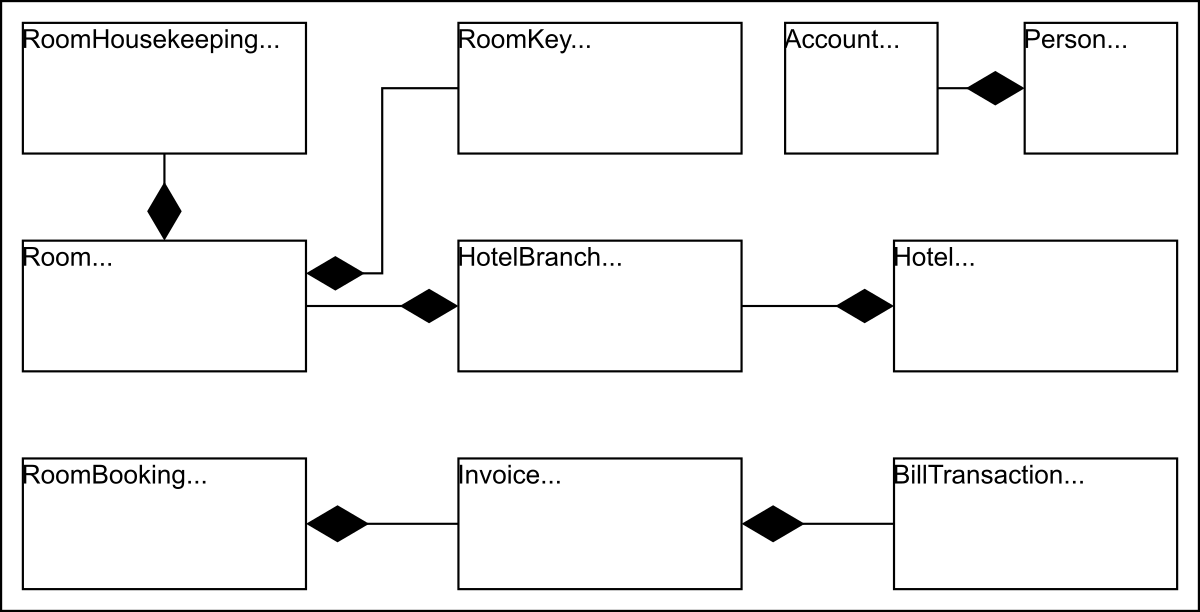
\includegraphics[width=0.5\textwidth]{Images/chapter_18/section_6101784200478720/6397020022767616.png}
 \caption{A composition relationship between classes}
\end{figure}

\subsubsection{Inheritance}\label{GrRDd34coTgbIpqCD8jOl-2}
\\
The following classes show an inheritance relationship:

\begin{itemize}
\item
\protect\phantomsection\label{LNjSNXtmMfDwCFEdKnndw}
\texttt{Receptionist}, \texttt{Guest}, and \texttt{Housekeeper} classes extend the \texttt{Person} class.
\item
\protect\phantomsection\label{bBi44hMfWmJDhnc6lsiub}
\texttt{Amenity}, \texttt{RoomService}, and \texttt{KitchenService} classes extend the \texttt{Service} class.
\item
\protect\phantomsection\label{fUTL88BzgvW8G2PAi2rQG}
Both \texttt{PostalNotification} and \texttt{EmailNotification} classes extend the \texttt{Notification} class.
\item
\protect\phantomsection\label{ZPApGdQQpCwjaeYGTqkNW}
The \texttt{Catalog} class implements the \texttt{Search} interface.
\end{itemize}
\begin{quote}
\textbf{Note:} We have already discussed the inheritance relationship between classes in the component section above one by one.
\end{quote}
\subsection{Class diagram of the hotel management system}\label{W0nuQJv6sS971g9ujUKFo}
\\
This section outlines the multiplicity (cardinality) relationships between the main classes in our hotel management system. We explain the allowed number of instances on each side for each relationship and the real-world or design rationale behind the connection. Understanding these relationships is key to modeling how different entities interact and collaborate to support key workflows in the system.

\begin{table}[h!]
\centering
\begin{tabular}{|p{3.5cm}|p{3.5cm}|p{3cm}|p{6.5cm}|}
\hline
\textbf{Source} & \textbf{Target} & \textbf{Multiplicity} & \textbf{Reason} \\
\hline
Hotel & HotelBranch & 1--0..* & A single hotel can have multiple branches across different locations. \\
\hline
HotelBranch & Room & 1--0..* & Each branch contains multiple rooms for booking. \\
\hline
Room & RoomBooking & 1--0..* & A room can be booked multiple times over its lifetime. \\
\hline
Guest & RoomBooking & 1--0..* & A guest may have multiple bookings over time. \\
\hline
Room & RoomMaintenance & 1--0..* & A room may undergo multiple maintenance sessions. \\
\hline
HouseKeeper & RoomMaintenance & 1--0..* & A housekeeper may be assigned to multiple room maintenance tasks. \\
\hline
RoomBooking & Notification & 1--0..* & Each booking can trigger multiple notifications (email or SMS). \\
\hline
RoomBooking & Invoice & 1--1 & Each booking results in exactly one invoice being generated. \\
\hline
Invoice & BillTransaction & 1--1..* & One invoice may involve one or more payment transactions. \\
\hline
Catalog & Room & 1--0..* & A catalog maintains a list of multiple rooms available for booking. \\
\hline
Room & RoomKey & 1--0..* & A room may have multiple keys (digital or physical). \\
\hline
Account & Person (Guest, etc.) & 1--1 & Each account is tied to exactly one person entity and vice versa. \\
\hline
\end{tabular}
\caption{Entity Relationships and Multiplicities in a Hotel Management System}
\label{tab:hotel_entity_relationships}
\end{table}


Here is the complete class diagram for our hotel management system:

\begin{figure}[htbp]
 \centering
 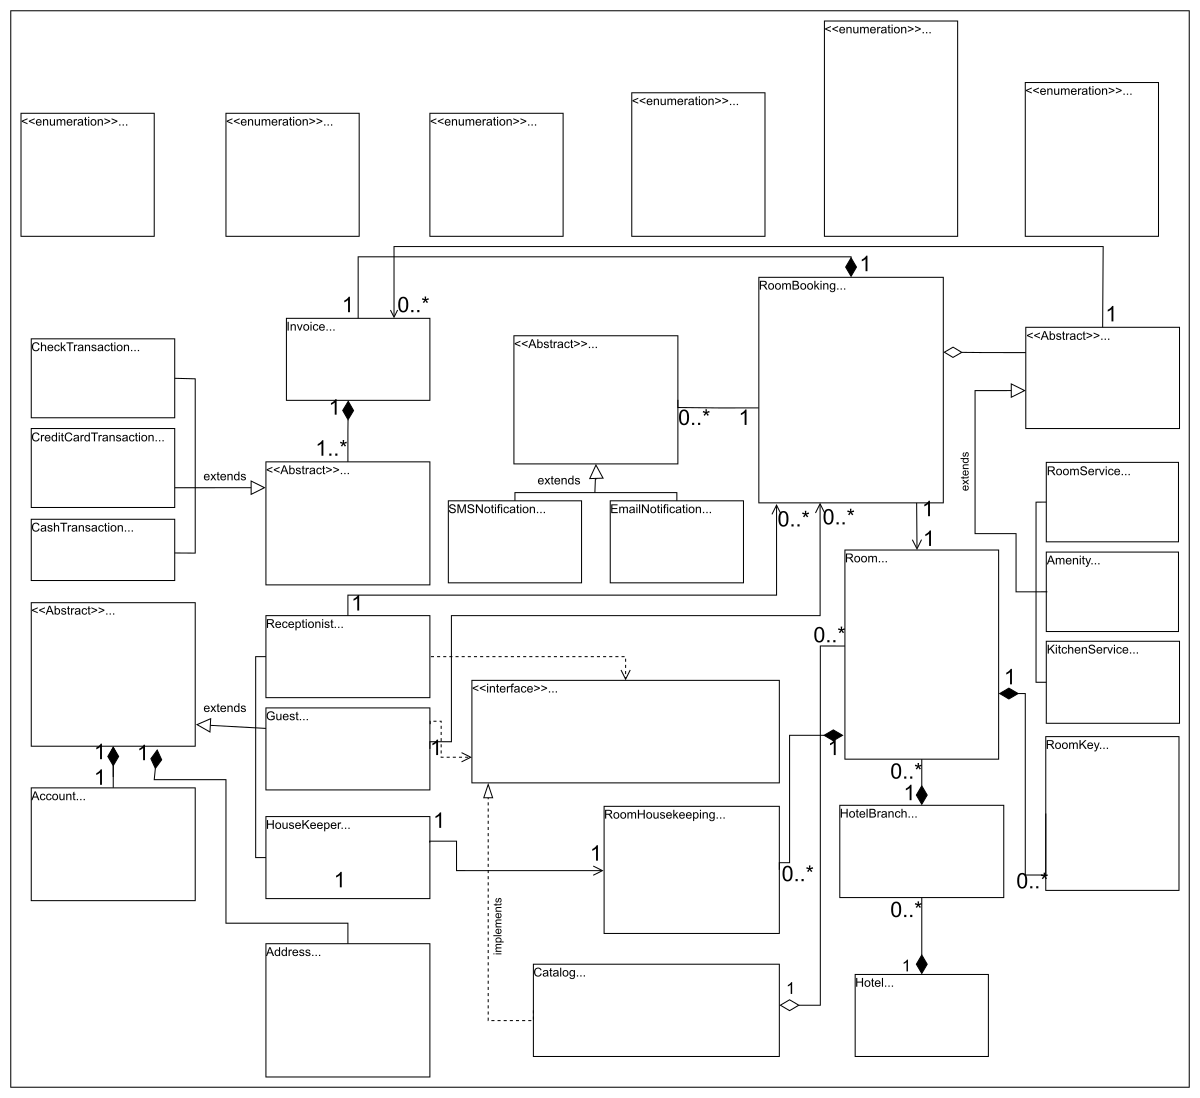
\includegraphics[width=0.5\textwidth]{Images/chapter_18/section_6101784200478720/5851520112132096.png}
 \caption{The class diagram of the hotel management system}
\end{figure}

\subsection{Design pattern}\label{e7G5uP-M0EJ1LWs4-Q-Vo}
\\
We apply the object-oriented design patterns based on system behavior to implement hotel management systems' core features in a flexible and scalable way.

\begin{itemize}
\item
The hotel system allows guests to receive notifications (like booking confirmations or reminders). The Observer design pattern can be used to model this behavior.
\item
The hotel system supports payment methods such as credit card, cash, and check. To handle this flexibly, we can use the Strategy design pattern.
\item
Booking confirmations may need to trigger different notifications (SMS or Email). We can use the Factory design pattern to manage these interchangeable notification types.
\item
We know that each payment type (cash, credit, check) follows a similar flow, but with some specific steps. We can use the Template Method design pattern to structure this reusable logic.
\item
We know that the catalog needs to manage and search through a collection of individual room objects. We can use the Composite design pattern to treat individual and grouped room operations uniformly.
\item
We know that the catalog or hotel instance should be globally accessible and should not have multiple copies. To enforce a single instance, we can use the Singleton design pattern.
\item
Room bookings and invoices involve setting multiple details, such as dates, rooms, guests, and status. The Builder design pattern can help us manage this complex construction clearly and safely.
\item
We know that components like notification services or payment processors might change or need mocking in tests. To make the system more flexible and testable, we can use Dependency Injection.
\end{itemize}

\subsection{AI-powered trainer}\label{5h3Jmj2lqIsj4A2I8nvPM}
\\
At this stage, everything should be clear. If you encounter any confusion or ambiguity, feel free to utilize the interactive AI-enabled widget below to seek clarification. This tool is designed to help you strengthen your understanding of the concepts.

\begin{figure}[htbp]
 \centering
 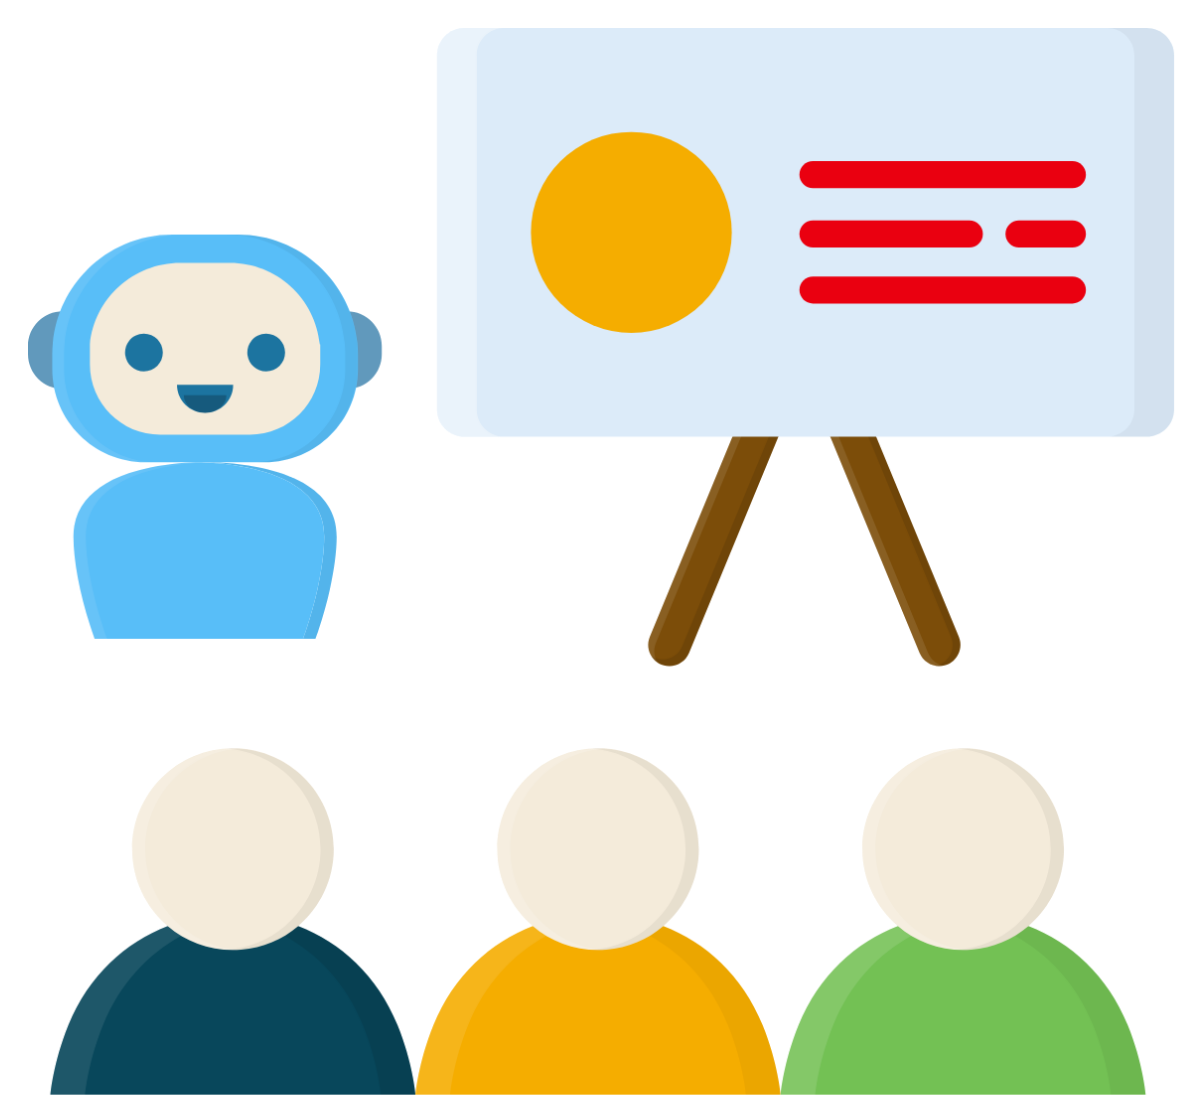
\includegraphics[width=0.15\textwidth]{Images/chapter_18/section_6101784200478720/6459295292850176.png}
 
\end{figure}

\subsection{Additional requirements}\label{QAbDdh23qLkrQrHukrHgI}
\\
The interviewer can introduce some additional requirements in the given hotel management system, or they can ask some follow-up questions. Let 's see examples of the additional requirements:
\\
\textbf{Discount:} Depending on special events such as the New Year, branch opening, a discount will be applied to the payment. The class diagram provided below shows the relationship of \texttt{Discount} with the \texttt{BillTransaction} class:

\begin{figure}[htbp]
 \centering
 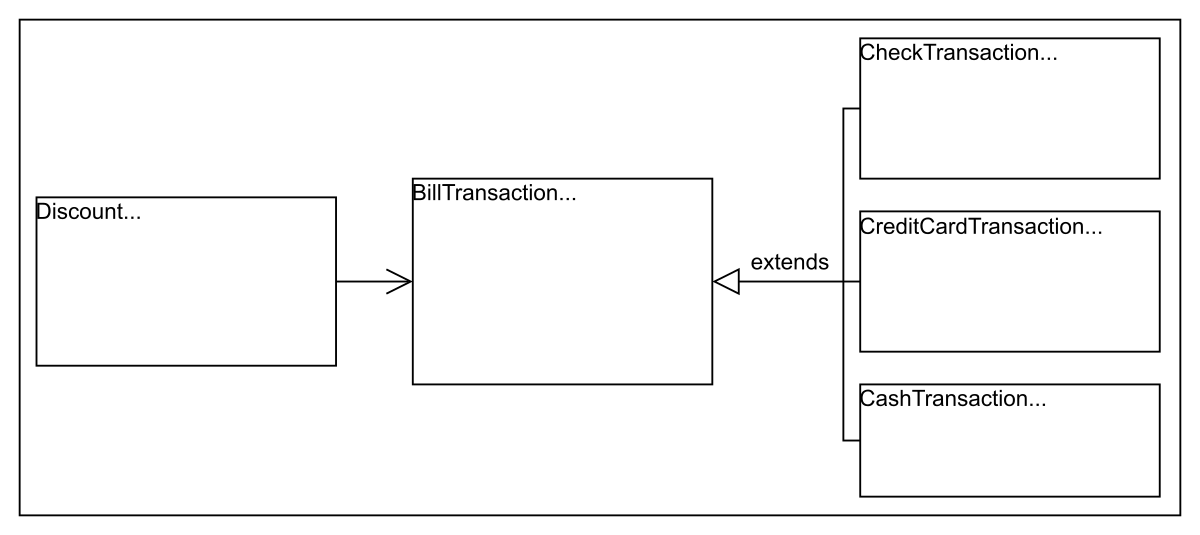
\includegraphics[width=0.5\textwidth]{Images/chapter_18/section_6101784200478720/5946243273326592.png}
 \caption{The relationship of the Discount class with the BillTransaction class}
\end{figure}

We have successfully designed the class diagram for the hotel management system. Let 's move to the next lesson to see how we can construct the sequence diagram for the system.

% End of section content